\documentclass{beamer}

\mode<presentation>{
\usetheme{Boadilla}
}

\setbeamertemplate{footline}[page number]

\usepackage[utf8]{inputenc}
\usepackage[ngerman]{babel}
\usepackage{graphicx}
\usepackage{multirow}
\usepackage{array}
\usepackage{colortbl}	

\usepackage{xcolor}
\usepackage{tikz} %Zeichnungen

\definecolor{darkblue}{rgb}{0, 0, 0.4}
\definecolor{cornellred}{rgb}{0.7, 0.11, 0.11}

\title[Elektrizitätslehre]{LCR-Schwingkreis und gekoppelte LC-Schwingkreise}
\author{Simon Schwarz}
\institute{Grundpraktikum Physik Teil I}
\date{25. September 2019}


\begin{document}

%Titelseite
\begin{frame}
\titlepage
\end{frame}

%Inhaltsverzeichnis
\begin{frame}
\frametitle{Inhalt}
\tableofcontents
\end{frame}


\section{LCR-Schwingkreis}
\subsection{Theorie}

\begin{frame}
\frametitle{Die Differentialgleichung des LCR-Schwingkreises}

\begin{columns}[c]
\column{.7\textwidth}

Kirchhoffsche Maschenregel: $U_0 = U_R + U_L + U_C = R\cdot I + L\frac{dI}{dt} + \frac{Q}{C}$ \\
Mit $I = \frac{dQ}{dt}$ folgt:
\begin{block}{Differentialgleichung (Gedämpfte Schwingung)}
$$L\frac{d^2Q}{dt^2} + R \frac{dQ}{dt} + \frac{Q}{C} = U_0$$ \\
$$\Leftrightarrow \frac{d^2Q}{dt^2} + 2\delta \frac{dQ}{dt} + \omega_0^2Q = \frac{U_0}{L}$$ \\
mit $\delta = \frac{R}{2L}$ und $\omega_0 = \frac{1}{\sqrt{LC}}$.
\end{block}

\column{0.25\textwidth}
\begin{figure}
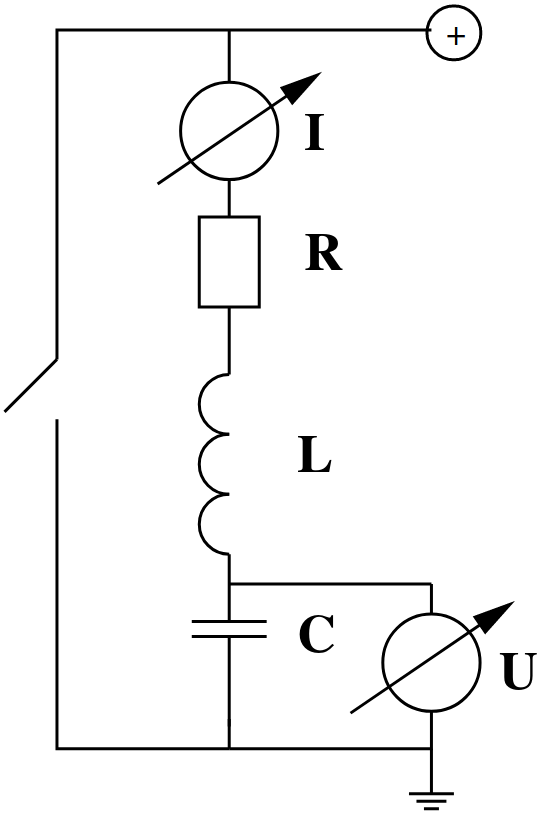
\includegraphics[width = \textwidth]{abbildungen/lcr_schaltbild.png}
\caption{Schaltbild des LCR-Schwingkreises}
\end{figure}
\end{columns}

\end{frame}


\begin{frame}
\frametitle{Lösungen der Differentialgleichung 1}
Bestimmbar über homogene und partikuläre Lösung.
Eigenschaften der Lösung sind abhängig von $\delta$ und $\omega_0$:
\begin{itemize}
\item $\delta < \omega_0$: Schwingfall
\item $\delta = \omega_0$: Aperiodischer Grenzfall
\item $\delta > \omega_0$: Kriechfall
\end{itemize}
\end{frame}

\begin{frame}
\frametitle{Lösungen der Differentialgleichung 2}
\begin{figure}
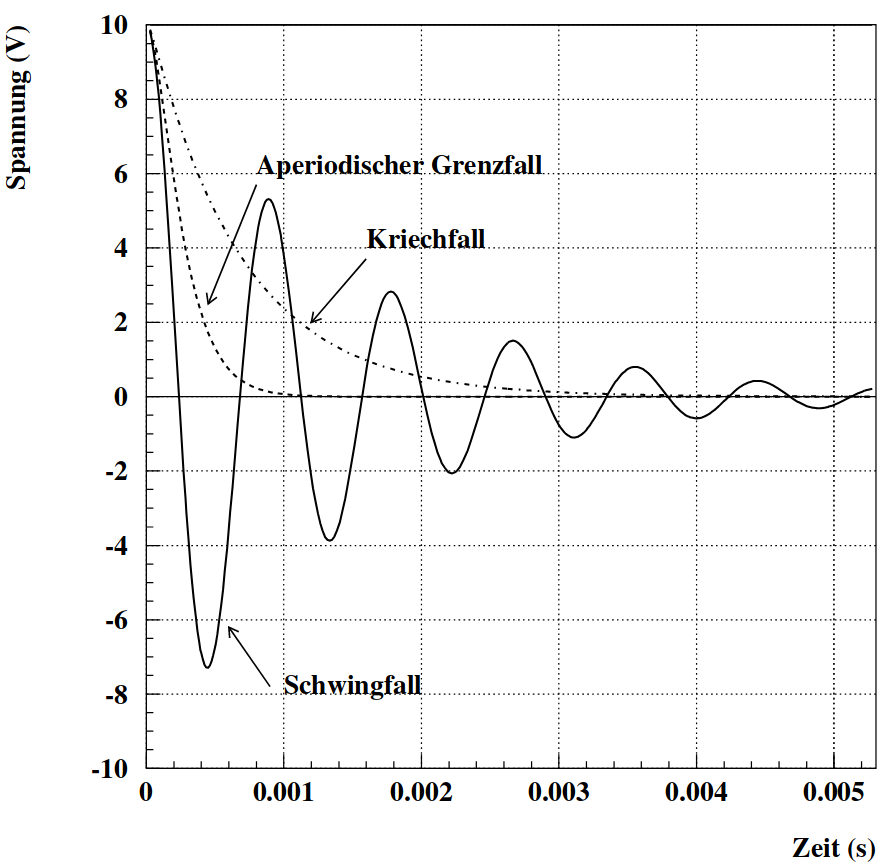
\includegraphics[scale = 0.25]{abbildungen/typen_schwingung.png}
\end{figure}
\end{frame}


\subsection{Versuchsaufbau}

\begin{frame}
\frametitle{Versuchsaufbau}
\begin{figure}
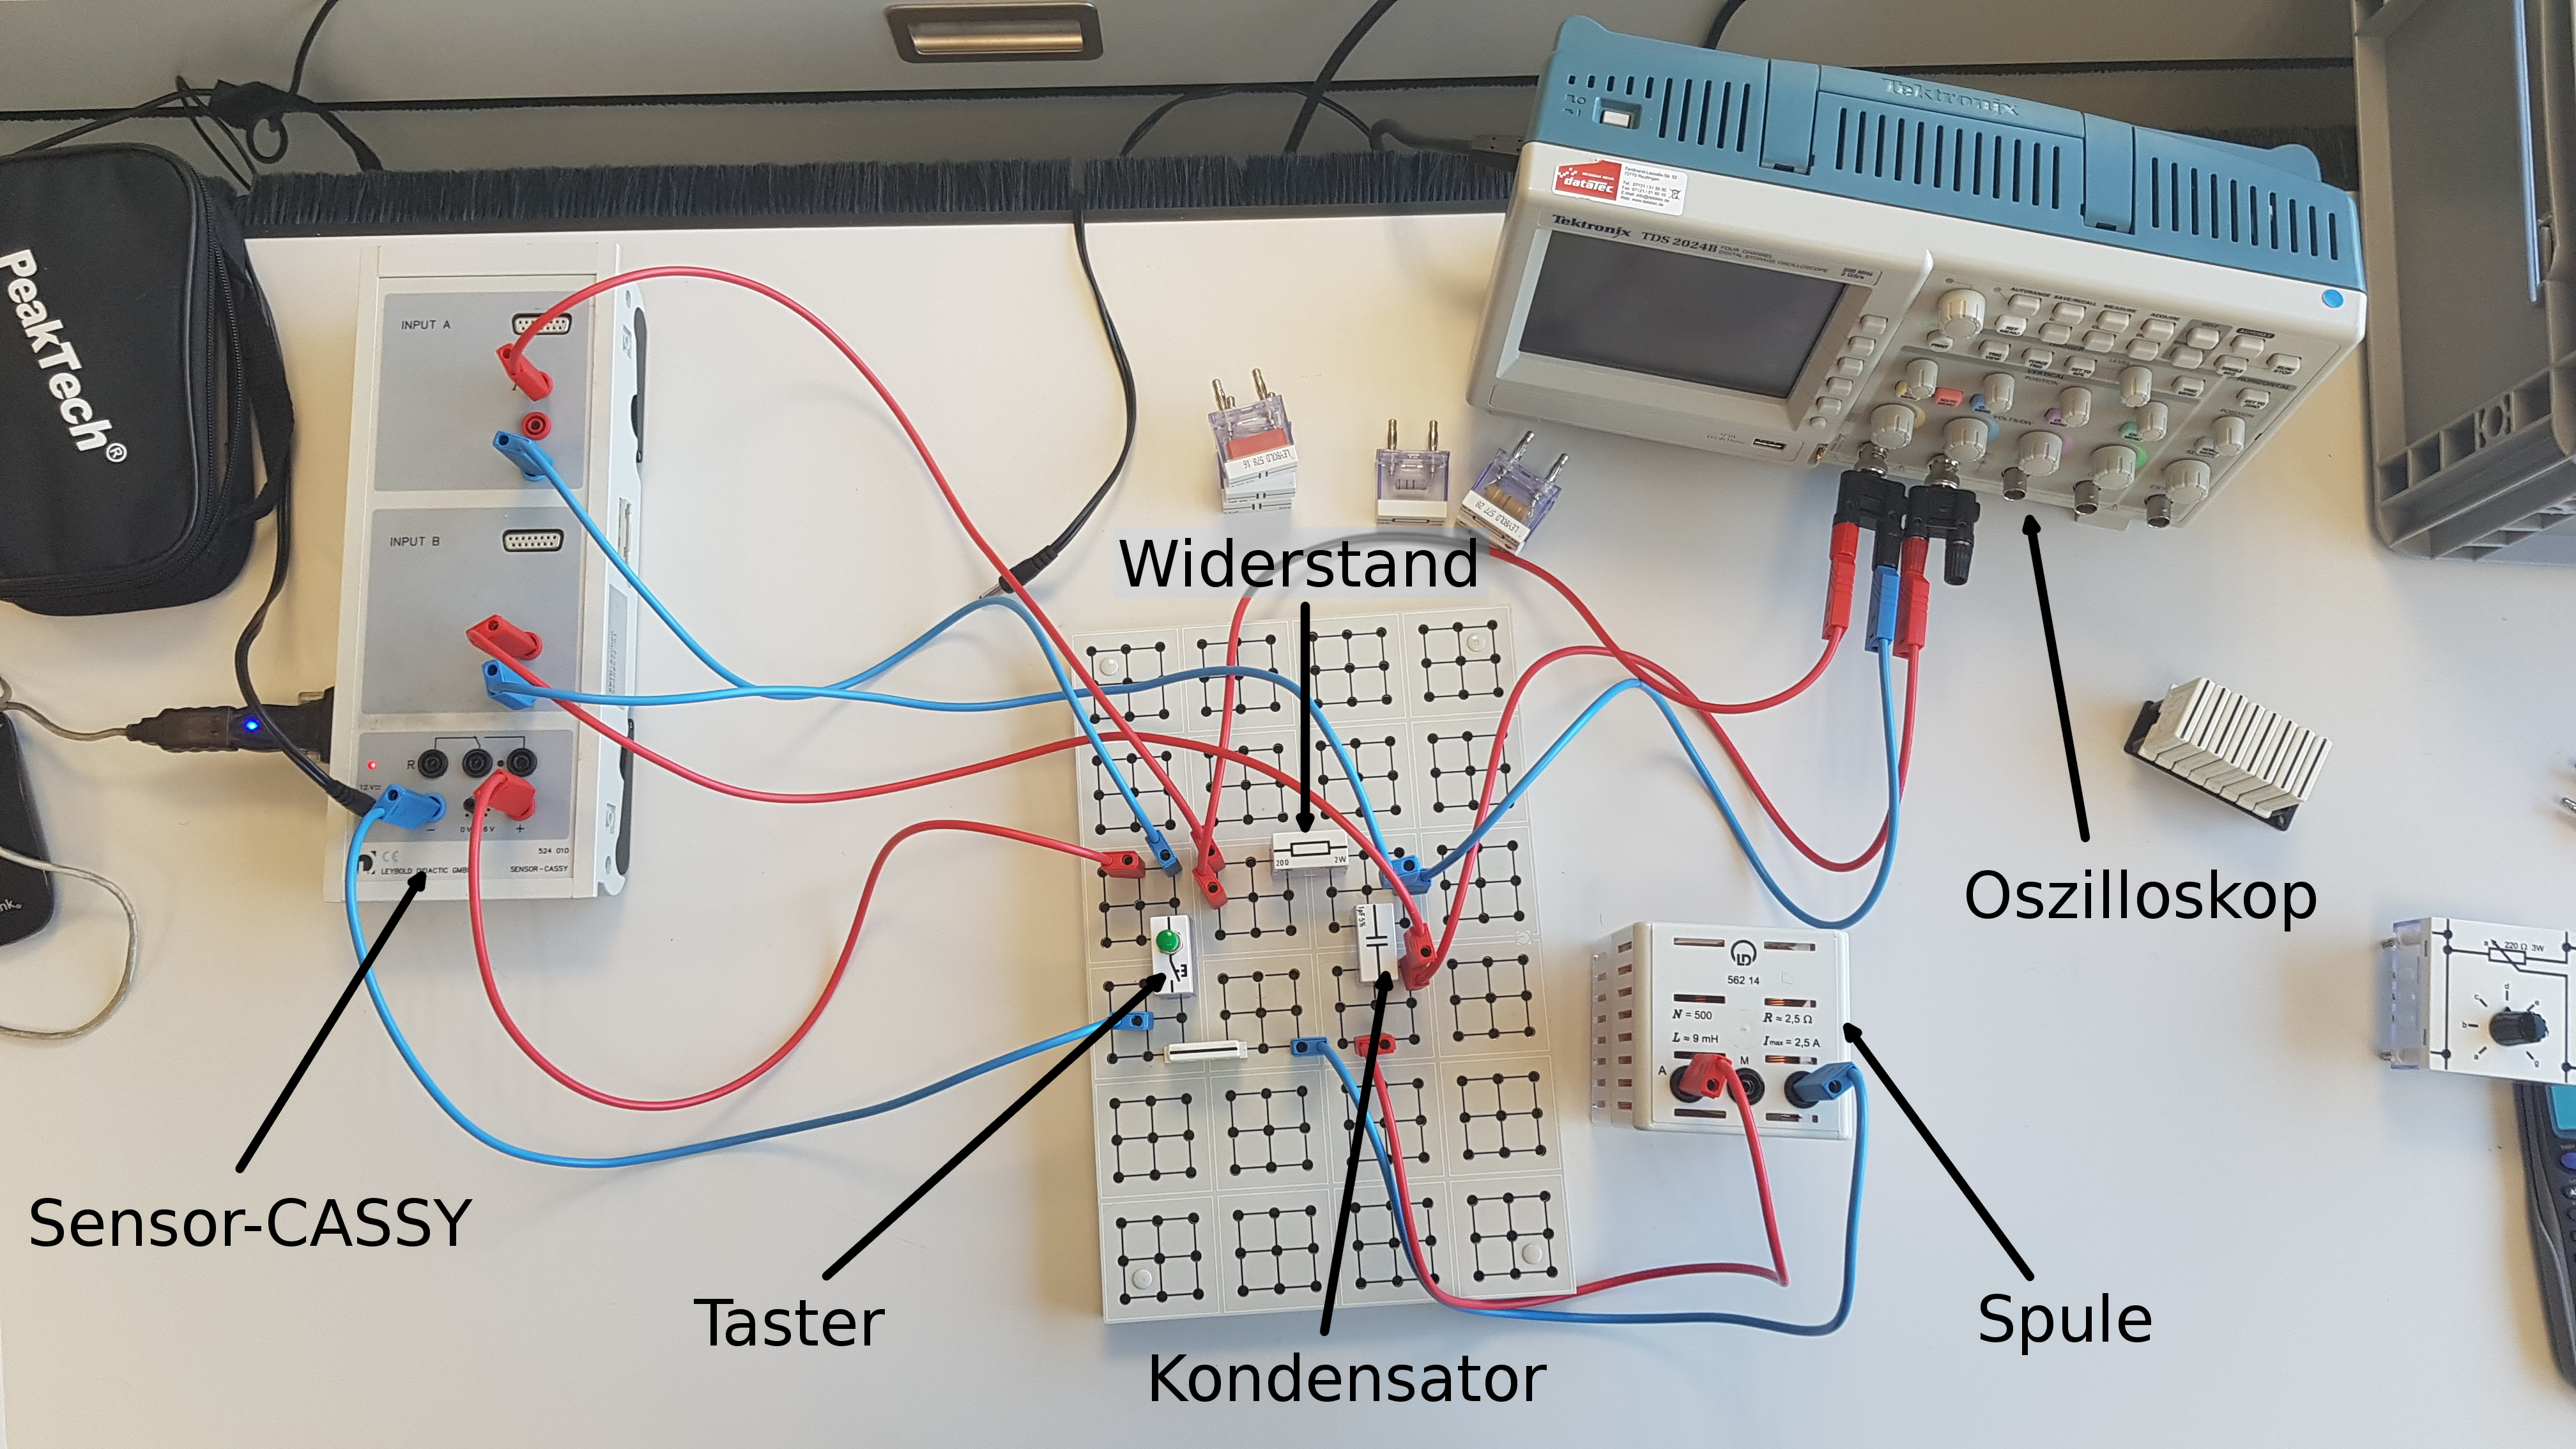
\includegraphics[width=\linewidth]{abbildungen/LCR_aufbau_beschriftet.jpg}
\end{figure}
\end{frame}


\subsection{Versuchsdurchführung}

\begin{frame}
\frametitle{Versuchsdurchführung}

\begin{enumerate}[-]
\item Widerstände unterschiedlicher Größe: 1$\Omega$, 5.1$\Omega$, 10$\Omega$, 20$\Omega$, [47$\Omega$ (nur Gruppe 2)], 100$\Omega$, 1000$\Omega$ und ein Potentiometer
\item Trigger zum Starten der Messreihe
\item 3 Messungen pro Widerstand
\item Messbereich: $\pm$ 3 V (Gruppe 1) oder $\pm$ 10 V (Gruppe 2)
\end{enumerate}

\begin{table}
\begin{tabular}{|c|c|c|c|c|}
\hline
\multirow{2}{*}{Messintervall} & \multicolumn{2}{c|}{Anzahl} & \multicolumn{2}{c|}{Messzeit} \\
\cline{2-5}
& Gruppe 1 & Gruppe 2 & Gruppe 1 & Gruppe 2 \\
\hline
10 $\mu$s & 8000 & 2000 & 80 ms & 20 ms \\
\hline
\end{tabular}
\caption{Messparameter}
\end{table}
\end{frame}

\subsection{Versuchsauswertung}

\begin{frame}
\frametitle{Versuchsauswertung}
\begin{figure}
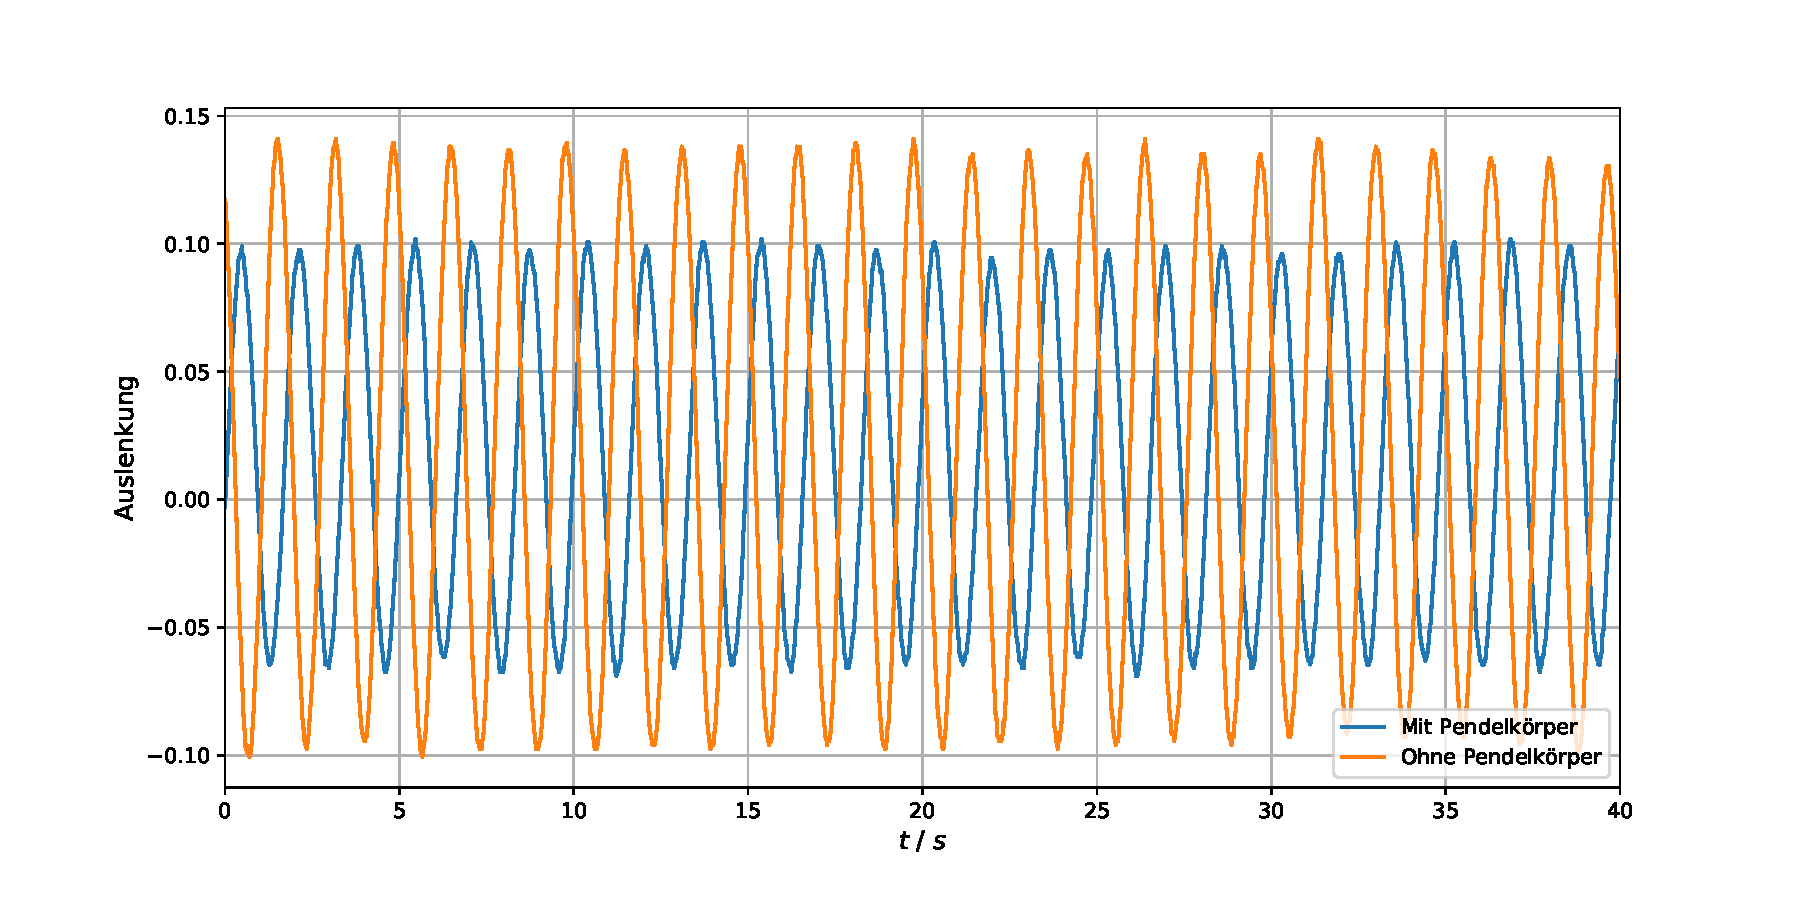
\includegraphics[width=.9\linewidth]{abbildungen/rohdaten.pdf}
\caption{Visualisierung der Schwingung mit einem Widerstand von $10\Omega$, $186\Omega$ und 1k$\Omega$.}
\end{figure}
\end{frame}

\subsubsection{Frequenzbestimmung}

\begin{frame}
\frametitle{Frequenzbestimmung}

\begin{figure}
\centering
%\includegraphics[width=0.8\textwidth]{plots/FFT.jpg}
\caption{FFT mit Peakfinder und Fehler}
\end{figure}

\end{frame}

\subsubsection{Dämpfungsbestimmung}

\begin{frame}
\frametitle{Dämpfungsbestimmung}

Modell: \hspace{0.2cm} $p(t) = Ae^{-\delta t} \sin(\omega t + \varphi) + B$

\begin{enumerate}[-]
\item Schätzung von $B$ nach dem Abklingen
\item Ablesen zweier Maxima (0.0029-0.029 hPa Ablesefehler)
\item $\delta = f\ln\left( \frac{p(t_0)-B}{p(t_1)-B} \right)$
\end{enumerate}

\begin{figure}
\centering
%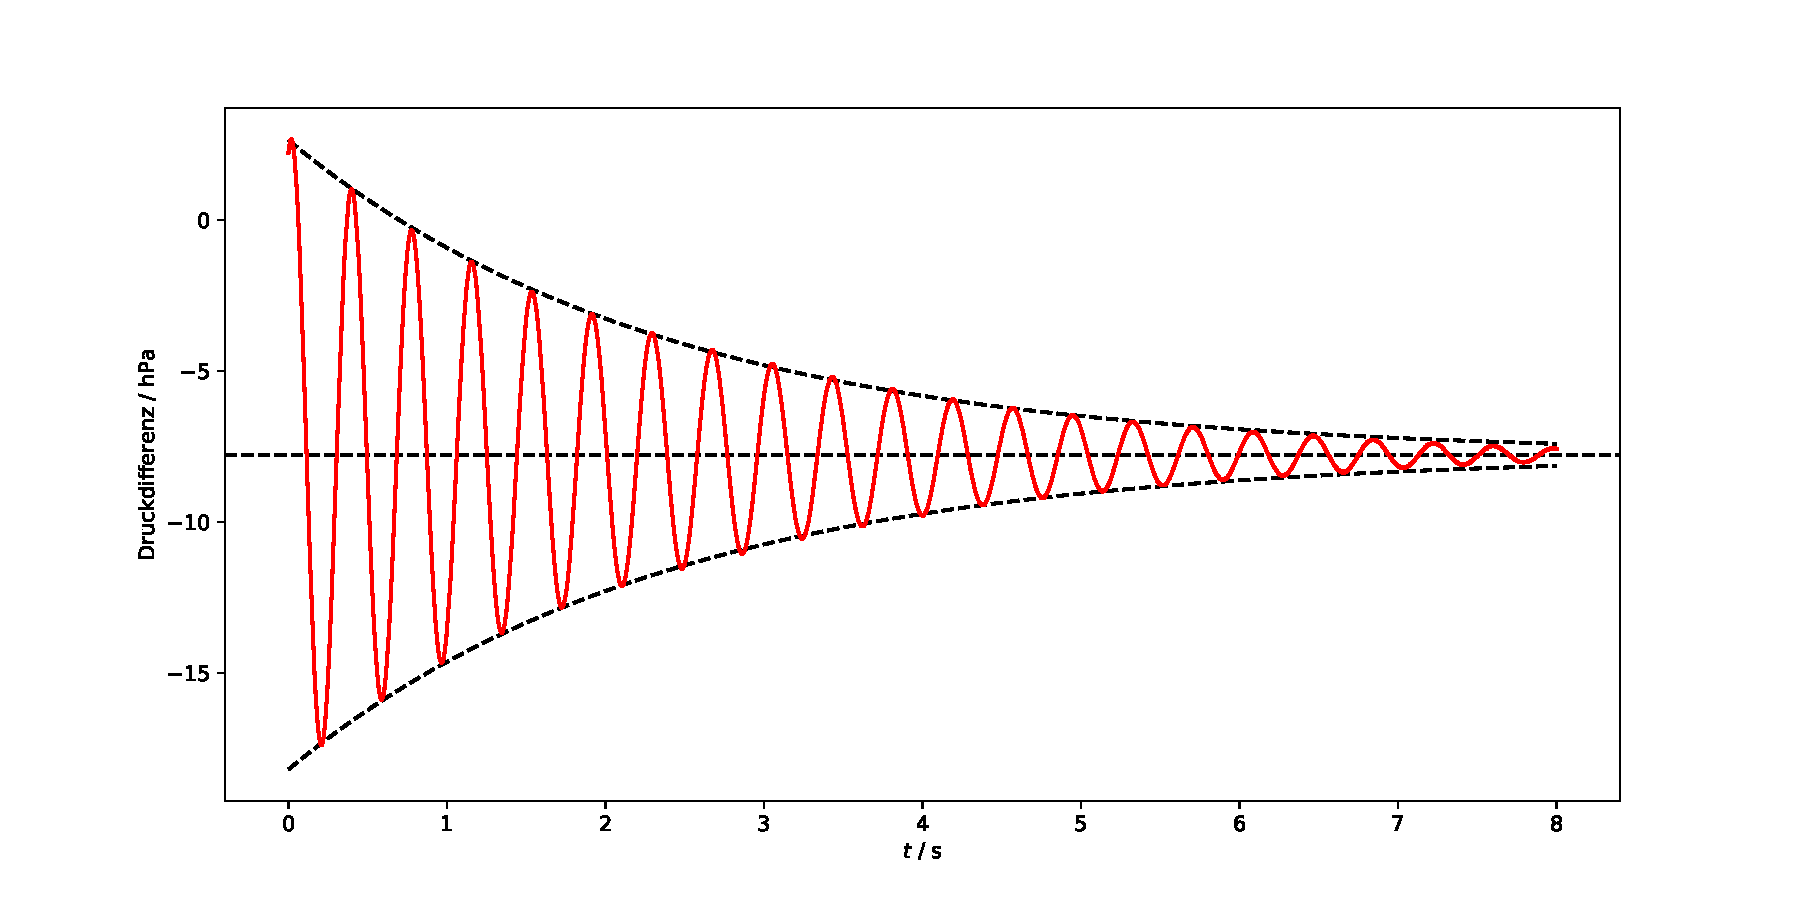
\includegraphics[width=0.9\textwidth]{plots/anpassung_delta.pdf}
\end{figure}

\end{frame}


\subsubsection{Volumenbestimmung}

\begin{frame}
\frametitle{Volumenbestimmung}

\begin{block}{Volumen}
$$V = V_F + x_0A + V_r$$
\end{block}

\begin{table}
\begin{tabular}{|c|c|c|c|}
\hline
\multirow{2}{*}{Flasche} & \multicolumn{2}{c|}{Volumen $V_F$ / $10^{-6}\mathrm m^3$} & \multirow{2}{*}{Fehler $\sigma$ / $10^{-6}\mathrm m^3$} \\
\cline{2-3}
& Gruppe 1 & Gruppe 2 & \\
\hline
 kleine & 307.8 & 309.7 & 1\\
\hline
mittlere & 1139.6 & 1119.1 & 1\\
\hline
große & 11267 & 11315 & 50\\
\hline
\end{tabular}
\end{table}

\begin{block}{Lineare Regression}
$$(V_F+x_0A)\left( \frac 1{\omega_0^2} \right) = \frac{p\kappa A^2}m \frac 1{\omega_0^2} - V_r$$
\end{block}

\end{frame}


\begin{frame}
\frametitle{Volumenbestimmung}

\begin{figure}
\begin{minipage}[t]{0.49\linewidth}
\centering
%\includegraphics[width=\linewidth]{plots/modell_2.jpg}
\end{minipage}
\hfill
\begin{minipage}[t]{0.49\linewidth}
\centering
%\includegraphics[width=\linewidth]{plots/regression_2.jpg}
\end{minipage}
\end{figure}
Aus der Steigung: \hspace{0.2cm} $\kappa = 1.308 \pm 0.039$

\end{frame}


\begin{frame}
\frametitle{Volumenbestimmung}

\begin{figure}
\centering
%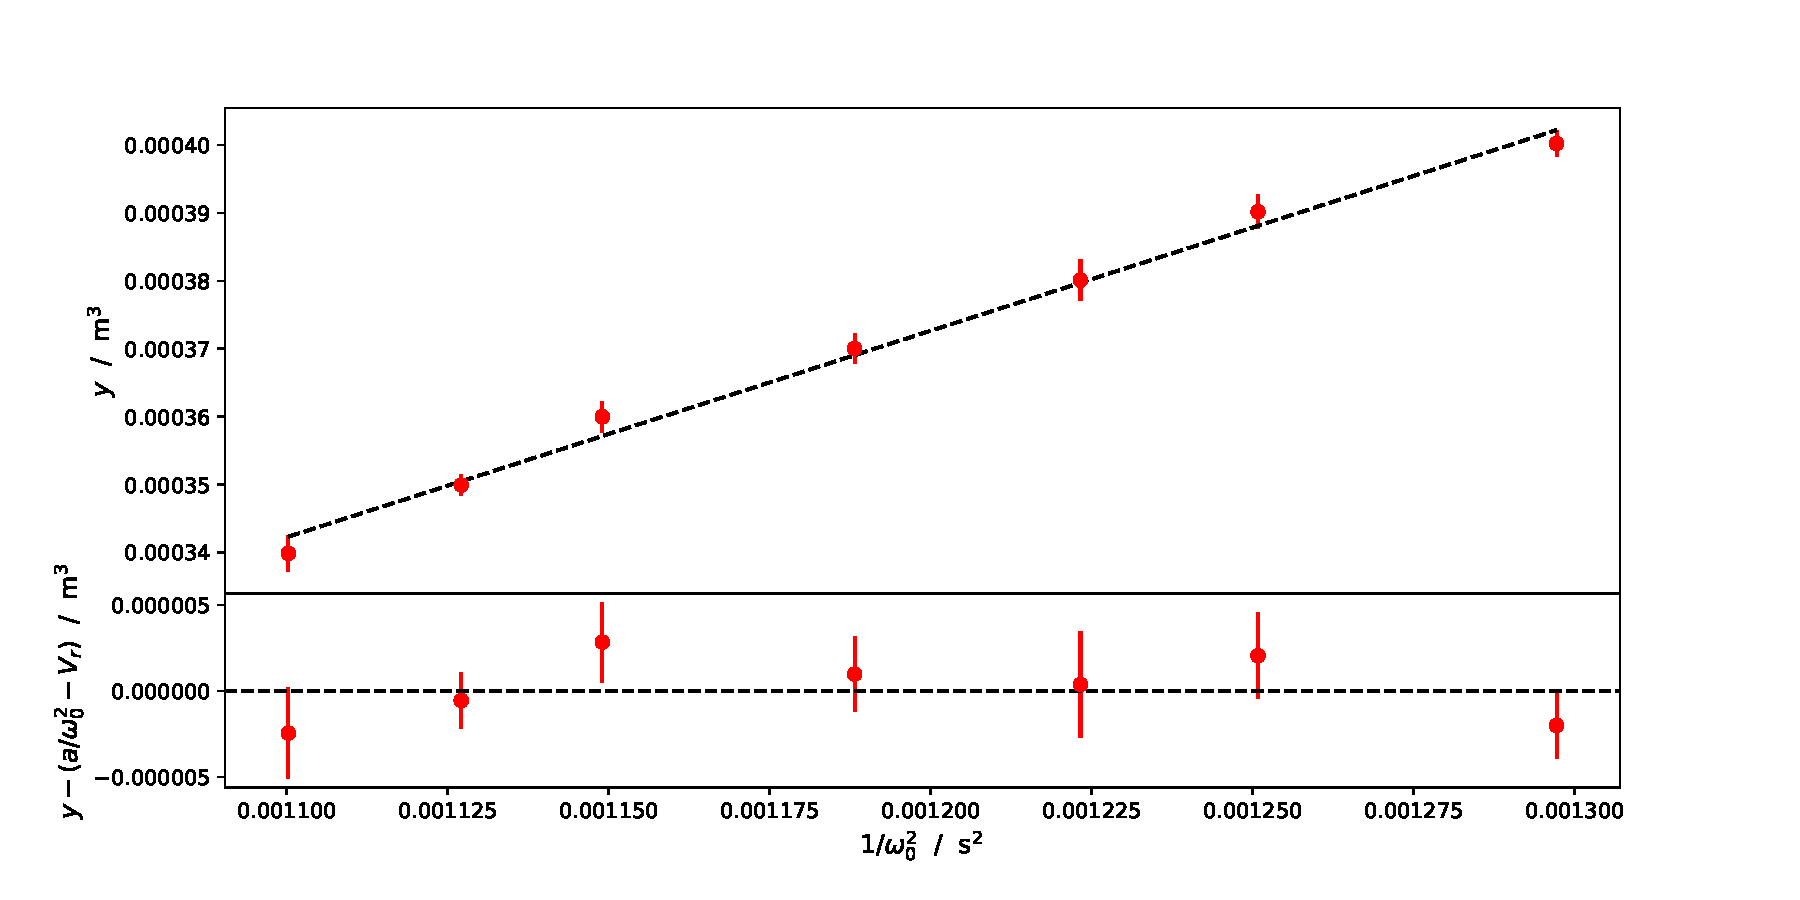
\includegraphics[width=0.9\linewidth]{plots/regression_kleine.pdf}
\end{figure}

\begin{table}
\begin{tabular}{|c|c|c|}
\hline
Steigung $a$ / $\frac{\mathrm m^3}{\mathrm s^2}$ & $V_r$ / $\mathrm m^3$ & $\frac{\chi^2}{n_{df}}$ \\
\hline
$0.304 \pm 0.012$ & $(-7.9 \pm 14.5) \cdot 10^{-6}$ & 0.88 \\
\hline
\end{tabular}
\end{table}

\end{frame}


\begin{frame}
\frametitle{Versuchsauswertung}

\begin{table}
\begin{tabular}{|c|c|c|}
\hline
Größe & Wert & Fehler $\sigma$ \\
\hline
Masse $m$ & 16.5 g & 0.03 g \\
\hline
Höhe $x_0$ & 0.15 bis 0.5 m & 0.003 m \\
\hline
Durchmesser $d$ & 16.00 mm & 0.003 mm \\
\hline
Außendruck $p_0$ & 994 hPa & 0.3 hPa \\
\hline
\end{tabular}
\caption{Restliche Größen mit Fehlern}
\end{table}
Bestimmung des Adiabatenkoeffizienten mittels
$$\kappa = \omega_0^2\frac{mV}{pA^2} = (\delta^2 + 4\pi^2 f^2) \frac{(V_F+x_0\frac{\pi}4 d^2 + V_r)}{(p_0+\frac{4mg}{\pi d^2})\frac{\pi^2d^4}{16}}$$
und Gaußscher Fehlerfortplfanzung.
\end{frame}




\begin{frame}
\frametitle{Versuchsauswertung}

Aus theoretischer Überlegung: \hspace{0.2cm} $\kappa_L = \frac 75 = 1.4$

\begin{table}
\begin{tabular}{|c|c|c|c|c|}
\hline
\multirow{2}{*}{Flasche} & \multicolumn{2}{c|}{$\kappa$} & \multicolumn{2}{c|}{$\frac{|\kappa-\kappa_L|}\sigma$} \\
\cline{2-5}
& Gruppe 1 & Gruppe 2 & Gruppe 1 & Gruppe 2 \\
\hline
\multirow{2}{*}{kleine} & $1.307 \pm 1.043$ & $1.266 \pm 0.019$ & \cellcolor[rgb]{0.06,1,0} 0.09 & 
\cellcolor[rgb]{1,0,0} 7.05 \\
\cline{2-5}
& $1.308 \pm 0.039$ & & \cellcolor[rgb]{1,0.48,0} 2.36 & \\
\hline
mittlere & $1.320 \pm 0.342$ & $1.337 \pm 0.007$ & \cellcolor[rgb]{0.16,1,0} 0.23 & \cellcolor[rgb]{1,0,0} 9.00 \\
\hline
große & $1.354 \pm 0.039$ & $1.494 \pm 0.003$ & \cellcolor[rgb]{0.79,1,0} 1.18 & \cellcolor[rgb]{1,0,0} 31.3 \\
\hline
\end{tabular}
\caption{Ergebnisse}
\end{table}

Mit gewichtetem Mittel und äußerem Fehler
\begin{table}
\begin{tabular}{|c|c|}
\hline
$\bar\kappa$ & $\frac{|\kappa-\kappa_L|}\sigma$ \\
\hline
$1.464 \pm 0.029$ & 2.21 \\
\hline
\end{tabular}
\end{table}


\end{frame}



\subsection{Fazit}

\begin{frame}
\frametitle{Fazit}

\begin{enumerate}[-]
\item Schlechte Ergebnisse mit großen Fehlern oder sehr großen Abweichungen von der Theorie
\item Schwierige Bestimmung von $V$ mittels Regression
\end{enumerate}
\end{frame}

\section{Gekoppelte LC-Schwingkreis}

\end{document}
